%
% HSR LaTex Template
% Copyright 2012, Florian Bentele / modified 2015 - Martin Stypinski
%
% Complete LaTex template for thesis at HSR, customized
% for Prof. Dr. Peter Heinzmann
%
%
% This document is free software: you can redistribute
% it and/or modify it under the terms of the GNU
% General Public License as published by the Free
% Software Foundation, either version 3 of the License,
% or (at your option) any later version.
%
% This document is distributed in the hope that it will
% be useful, but WITHOUT ANY WARRANTY; without even the
% implied warranty of MERCHANTABILITY or FITNESS FOR A
% PARTICULAR PURPOSE. See the GNU General Public
% License for more details.
%
% You should have received a copy of the GNU General
% Public License along with this document. If not, see
% <http://www.gnu.org/licenses/>.
%

\newcommand{\kiru}{Kirusanth Poopalasingam}
\newcommand{\styp}{Martin Stypinski}
\newcommand{\aeme}{Marcel Amsler}

\documentclass[11pt]{hsrthesis}

\makeindex

\makeglossaries
\newglossaryentry{Clusteranalyse}{
	name=Clusteranalyse,
	description={Ein Verfahren zur Feststellung von Ähnlichkeiten in Datenbeständen},
	first={Clusteranalyse}
}

\newglossaryentry{AMQP}{
	name=AMQP,
	description={ Advanced Message Queuing Protocol, wird verwendet für die Übertragung der Messages an RabbitMQ }
}

\newglossaryentry{APK}{
	name=APK,
	description={ Android Package, ist das Datenformat indem Android Apps gespeichert werden. }
}

\newglossaryentry{OTG}{
	name=OTG,
	description={ USB On-the-go, ist der Standard um eine direkte Kommunikation zwischen USB-Geräten ohne Host-Controller zu ermöglichen. In unserem Fall um ein USB Gerät an ein Smartphone anzuschliessen. }
}

\newglossaryentry{Message-Producer}{
	name=Message Producer,
	description={ Bei einem Messaging-System oder einer MOM (Message Oriented Middleware) gibt es immer Message Producer und Message Consumer. Ein Message Producer erstellt Nachrichten, ein Message Consumer hingegen empfängt und verarbeitet diese. }
}


\newglossaryentry{MAVLink}{
	name=MAVLink,
	description={ MAVLink ist ein reines Header-Protokoll, dass es ermöglicht unbemannte Fahr- und Flugzeuge zu kontrollieren. Es kann über verschiedene Protokolle laufen (USB, UDP, TCP) }
}

\newglossaryentry{Flight-Controller}{
	name=Flight-Controller,
	description={ Der Flight-Controller ist der Kern der Drohne, übernimmt die Stabilisierung und Steuerung der Rotoren. Wird über das MAVLink Protokoll mit Befehlen gesteuert. }
}

\newglossaryentry{CGAL}{
	name=CGAL,
	description={The Computational Geometry Algorithms Library ist eine C++ Bibliothek die einfachen und effizienten Zugang zu Algorithmen auf geometrischen Objekten ermöglicht. Sie bietet unter anderem folgende Algorithmen: ConvexHull, AlphaShape, MeshGeneration, ShapeAnalysis, uvm.}
}

\newglossaryentry{SFCGAL}{
	name=SFCGAL,
	description={Simple Feature CGAL ist eine Bibliothek die mit Geometrie Typen aus dem OGC Standart arbeitet. Es kann somit mit den bekannten Datentypen die im OpenSource GIS Umfeld weit verbreitet sind, gearbeitet werden.}
}

\newglossaryentry{OGC}{
	name=OGC,
	description={Open Geospatial Consortium ist eine Organisation die viele GIS relevante Standarts im Opensource bereich geschaffen hat.}
}

\newglossaryentry{MIT-Lizenz}{
	name=MIT-Lizenz,
	description={Eine Software-Lizenz, die es Jedem Erlaubt den Code in jeder Art weiterzuverwenden.}
}

\newglossaryentry{BEC}{
	name=BEC,
	description={Battery Eliminator Circuit ist eine im RC-Modellbau verwendete Terminologie für eine Spannungsstabilisierungsschaltung, um konstante Spannung zu gewährleisten.}
}

\newglossaryentry{Java Topology Suite}{
	name=Java Topology Suite (JTS),
	description={Java Topology Suite ist ein API für 2D Objekte und deren Operationen. Sie erfüllt den Open Geospatial Consortium Standard und implementiert somit die gleichen Objekte wie PostGIS.}
}

\newglossaryentry{CRUD}{
	name= CRUD,
	description={Abkürzung für C = Create, R = Read, U = Update, D = Delete. Es wird zur Bezeichnung von Operationen auf einem Model/Resource verwendet. Beispielsweise sollen Benutzer erstellt (Create), angesehen(Read), geändert (Update) und gelöscht (Delete) werden können.}
}





\begin{document}
\newcommand{\thesistitle}{Project Helin}
\newcommand{\thesisauthora}{Marcel Amsler}
\newcommand{\thesisauthorb}{Kirusanth Poopalasingam}
\newcommand{\thesisauthorc}{Martin Stypinski}
\newcommand{\professor}{Prof. Dr. Markus Stolze}
\newcommand{\thesistype}{Bachelorarbeit}
\newcommand{\departement}{Abteilung Informatik}
\newcommand{\school}{Hochschule für Technik Rapperswil}
\newcommand{\term}{Frühlingssemester 2016}
\newcommand{\thedate}{29. Mai 2015}
\newcommand{\timeperiode}{16.02.2015 - 29.05.2015}
\newcommand{\workload}{360 Stunden, 12 ECTS pro Student}
\newcommand{\linktothesis}{https://github.com/Project-Helin/}

\maketitle


\newpage

\pagenumbering{roman}


% The main content
%%%%%%%%%%%%%%%%%%


\addcontentsline{toc}{chapter}{Eigenständigkeitserklärung}
\chapter*{Eigenständigkeitserklärung}

%\chapter{Eigenständigkeitserklärung}
Wir erklären hiermit,
\begin{itemize}
	\item{dass wir die vorliegende Arbeit selber und ohne fremde Hilfe durchgeführt haben, ausser
derjenigen, welche explizit in der Aufgabenstellung erwähnt sind oder mit dem Betreuer
schriftlich vereinbart wurden,}
	\item{dass wir sämtliche verwendeten Quellen erwähnt und gemäss gängigen wissenschaftlichen
Zitierregeln korrekt angegeben haben,}
	\item{dass wir keine durch Copyright geschätzten Materialien (z. B. Bilder) in dieser Arbeit in
unerlaubter Weise genutzt haben.}
\end{itemize}
\begin{verbatim}




\end{verbatim}
Rapperswil, den \today
\begin{verbatim}







\end{verbatim}
%\includegraphics[width=1.1\textwidth]{images/signature.png}
\begin{tabular*}{\textwidth}{p{0cm}>{\centering\arraybackslash}m{4.8cm}>{\centering\arraybackslash}m{4.8cm}>{\centering\arraybackslash}m{4.8cm}p{0cm}}
	& Marcel Amsler & Kirusanth Poopalasingam & Martin Stypinski & \\
\end{tabular*}
\newpage
\addcontentsline{toc}{chapter}{Danksagung}
\chapter*{Danksagung}
Zunächst möchten wir uns an dieser Stelle bei all denjenigen bedanken, die uns während der Anfertigung dieser Arbeit unterstützt und motiviert haben.
\begin{itemize}
	\item{Mir findet dann scho öpert :)}
\end{itemize}
\newpage
\addcontentsline{toc}{chapter}{Abstract}
\chapter*{Abstract}
YOLO Abstract 1
\newpage
\addcontentsline{toc}{chapter}{Management Summary}
\chapter*{Management Summary}
\section*{Ausgangslage}

\section*{Ergebnisse}

\section*{Ausblick}

\newpage
\addcontentsline{toc}{chapter}{Aufgabenstellung}
\chapter*{Aufgabenstellung}
\label{cha:aufgabenstellung}

\section*{Betreuer}
\begin{itemize}
	\item Prof Dr. Markus Stolze, Dozent für Informatik HSR
\end{itemize}

\section*{Ausgangslage, Problembeschreibung}
\lipsum[2-3]

\section*{Aufgabenstellung}
\lipsum[2-3]

\section*{Termine}
Die Termine ergeben sich aus den Semesterterminen der HSR (Bachelorstudium).

% Table of content
% % % % % % % % %
\newpage
\addcontentsline{toc}{chapter}{Inhaltsverzeichnis}
\tableofcontents
\newpage

\pagenumbering{arabic}
\setcounter{page}{1}



\part{Technischer Bericht}
\newpage
\chapter{Umsetzung}

\section{Multicopter Hardware}

Um unsere Plattform testen zu können, haben wir zwei identische Quadcopter aufgebaut.
Wichtig dabei ist, dass für die Benutzung unserer Plattform kein identischer Aufbau nötig ist. Es wird lediglich ein Flight-Controller mit einer MAV-Link kompatiblen Firmware benötigt. z.B. ArduCopter, PX4, usw. 

\subsection{Frame und Antrieb}

Der Frame, die Motoren und ESCs wurden als Kit gekauft. Es handelt sich dabei um ein DJI Flamewheel 450 Frame mit DJI 2312 960kV Motoren und ESeries 420 20A ESCs. Dieses Kit ist weltweit gut verfügbar und deshalb ideal geeignet um einen Versuchsaufbau zu erstellen.

\begin{figure}[h]
	\centering
	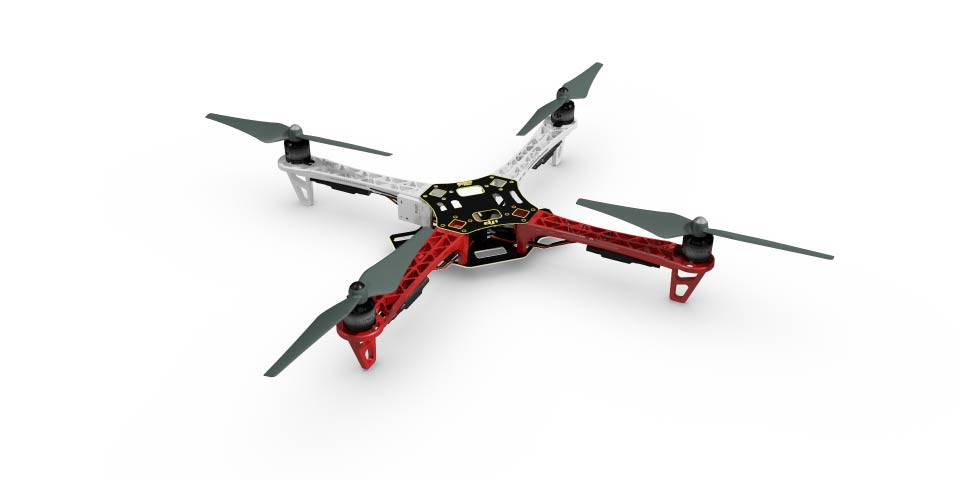
\includegraphics[width=0.9\textwidth] {images/hardware/f450.jpg} 
	\caption{DJI F450 Flamewheel Kit}
	\label{fig:f450}
\end{figure}


\subsection{Flight-Controller}

Der Flight-Controller ist das Herzstück eines Quadcopters. Im Unterschied zu anderen Ferngesteuerten Fahr- und Flugzeugen kann ein Multicopter nur über ein Fly-by-Wire System kontrolliert werden. Das heisst alle Befehle, die von der Fernbedienung kommen, müssen interpretiert und umgewandelt werden, damit die Motoren eine Bewegung in die gewünschte Richtung zu erzeugen können. In Kombination mit einem GPS Modul (Abb. \ref{fig:gps-module}) ermöglich der Controller verschiedene Flugmodi, wie beispielsweise das Schweben an einem Punkt oder automatisches abfliegen von Wegpunkten.

Als Flight-Controller setzen wir ein Pixhawk ein. Es ist sehr vielseitig und kann gut mit zusätzlichen Sensoren erweitert werden, ausserdem unterstützt es gängige Firmwares, die auch auf günstigeren Controllern laufen. Als Firmware für das Pixhawk setzen wir ArduCopter ein, da sie komplett Open-Source ist und auch bei vielen anderen Projekten eingesetzt wird. Sie unterstützt ausserdem das MAV-Link Protokoll, das es ermöglicht verschiedene Hardware über den USB Port anzusprechen.

\begin{figure}[h]
	\centering
	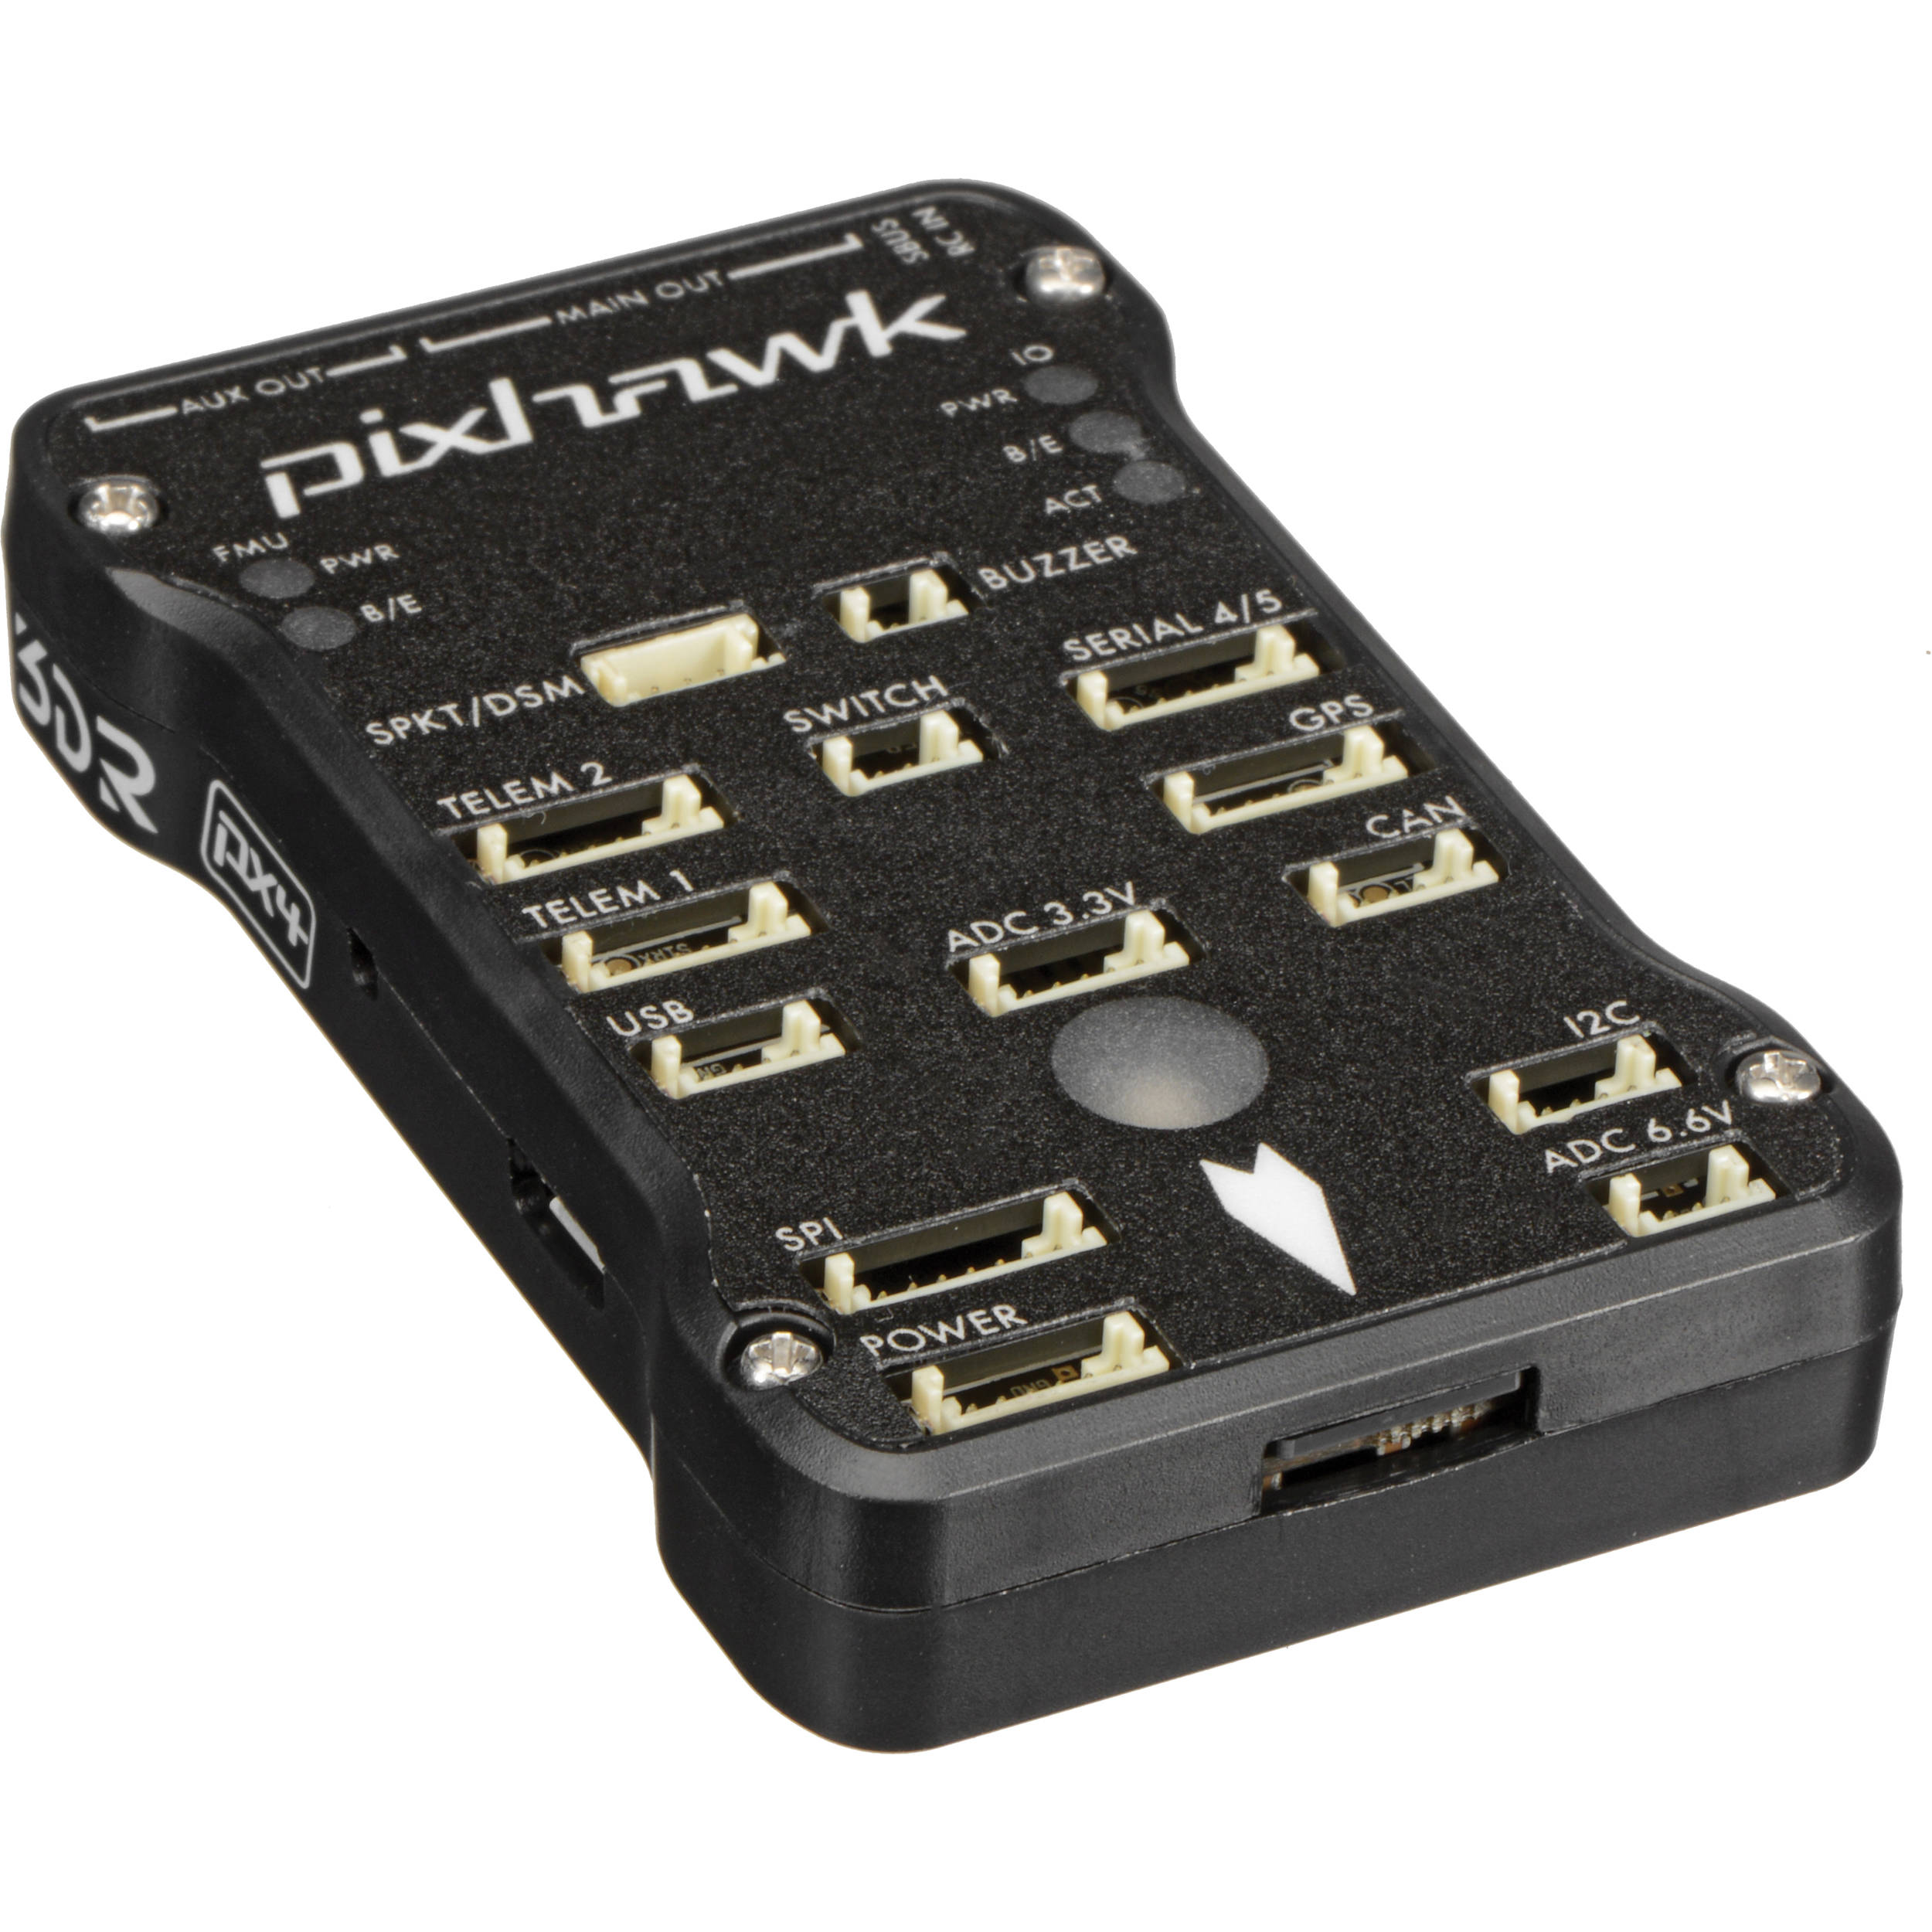
\includegraphics[width=0.3\textwidth] {images/hardware/pixhawk.jpg} 
	\caption{Pixhawk Flight-Controller}
	\label{fig:pixhawk}
\end{figure}

\begin{figure}[h]
	\centering
	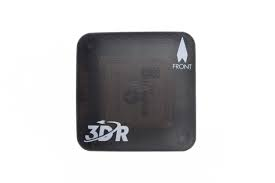
\includegraphics[width=0.3\textwidth] {images/hardware/gps-module.jpg} 
	\caption{GPS-Modul für Pixhawk}
	\label{fig:gps-module}
\end{figure}

\subsection{Ausbaustufen}

Während des Projekts wurden die Hardware laufend den Bedürfnissen angepasst. Daher gibt es mehrere Prototypen, die für die Versuche genutzt wurden.

\subsubsection{Prototyp 1}

Um das Zusammenspiel der Hardwarekomponenten zu testen und erste Versuche mit dem GPS und den verschiedenen Flugmodi zu sammeln, wurde sehr schnell ein Prototyp gebaut.

\begin{figure}[h]
	\centering
	\includegraphics[width=0.9\textwidth] {images/hardware/prototype1.jpg} 
	\caption{Erster Prototyp ohne Landegestellt und ohne Smartphone}
	\label{fig:prototyp-1}
\end{figure}






\part{Anhang}
\newpage
\renewcommand \thechapter{\Alph{chapter}}


\chapter{Projektplan}
\section{Änderungsgeschichte}
\begin{tabularx}{\textwidth}{|c|c|X|c|}
  \hline
  \textbf{Datum} & \textbf{Version} & \textbf{Änderung} & \textbf{Autor} \\
  \hline \hline
  26.02.2016 & 1.0 & Erstellen des Projektplans & Martin Stypinski \\
  \hline
\end{tabularx}

\section{Einleitung}
\subsection{Ziel und Zweck}
Ziel dieser Arbeit ist \textit{Project-Helin} umzusetzten. 

\subsection{Lieferumfang}
Der Lieferumfang dieser Arbeit entspricht den Vorgaben der HSR:
\begin{itemize}
	\item{Zu Handen des Betreuers:
	\begin{itemize}
		\item{Ein gedrucktes Exemplar der Dokumentation}
		\item{Dokumentation, sämtliche Dokumente und Sourcen auf CD}
	\end{itemize}}
	\item{Poster - Enthält Zusammenfassung der Arbeit}
	\item{Abstract für die Bachelorarbeitsbrochure}
\end{itemize}
Zusätzlich ist es uns ein Anliegen, dass der Sourcecode und die Erfahrungen über den Zeitraum der Bachelorarbeit hinaus bestehen bleiben. Daher wurde ein github-repository eingerichtet, dass nach beendigung der Arbeit sämtliche Teile enthält: \textbf{\url{https://github.com/Project-Helin}}

\subsection{Annahmen und Einschränkungen}
Es kann angenommen werden, dass der Zeitplan im Rahmen der regulären Bachelorarbeit Zeit gültig ist. Es wird dabei berücksichtigt das ein Zeithorizont von 17 Wochen zuverfügung steht und die maximale Arbeitszeit von 360 Stunden pro Person nicht überschritten werden soll.

\newpage

\section{Projektorganisation}
\subsection{Organisationsstruktur}

\begin{figure}[ht]
%\begin{figure}[H]
	\centering
	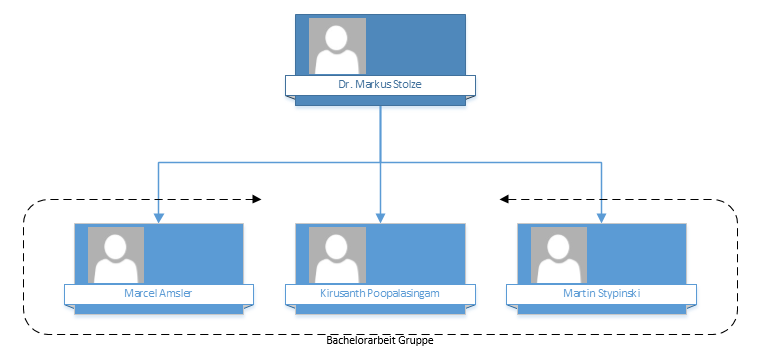
\includegraphics[width=\textwidth]{images/organigram.png}
	\caption{Grobübersicht über den Projektplan}
	\label{Risk result}
\end{figure}

\begin{tabularx}{\textwidth}{|c|c|X|}
  \hline
  \textbf{Name} & \textbf{E-Mail} & \textbf{Verantwortung} \\
  \hline \hline
  Prof. Dr. Markus Stolze & \url{markus.stolze@hsr.ch} & Betreuer der Arbeit\\
  \hline \hline
  Marcel Amsler & \url{marcel.amsler@hsr.ch} & \\
  \hline
  Kirusanth Poopolasingam & \url{kirusanth.poopalasingam@hsr.ch} & \\
  \hline
  Martin Stypinski & \url{martin.stypinski@hsr.ch} & \\
    \hline
\end{tabularx}

\newpage

\section{Meilensteinplanung}
Grundsätzlich wird während der gesammten Arbeit Scrum als Projektmanagement eingsetzt. Ein Scrum-Sprint dauer in der Regel 2 Wochen. Die Meilensteine helfen nur zu definieren welche Tasks prioritär behandelt werden sollen.

\begin{figure}[ht]
%\begin{figure}[H]
	\centering
	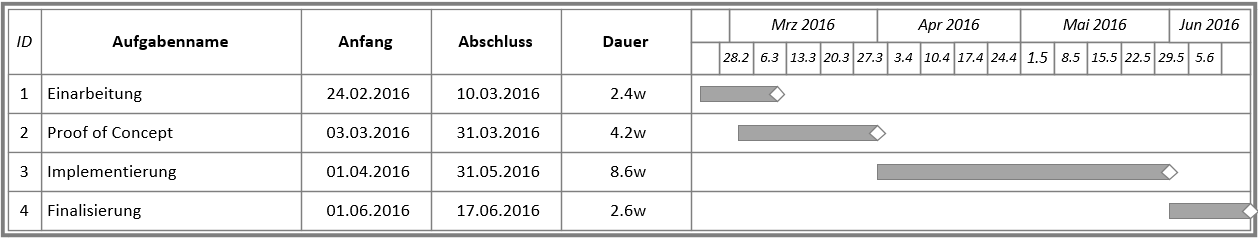
\includegraphics[width=\textwidth]{images/projplan.png}
	\caption{Grobübersicht über den Projektplan}
	\label{Risk result}
\end{figure}


\begin{itemize}
	\item{\textbf{Ende der Einarbeitung:} 
		\begin{itemize}
			\item{\textbf{Datum:} 10.03.2015}
			\item{\textbf{Ziel:} Entwicklungsumgebund und Prozesse stehen.}
			\item{\textbf{Erfüllungskriterium:} Sämtliche prozessbegleitenden Massnahmen sind lauffähig. Es kann gemäss den Anforderungen automatisch deployt werden.}
		\end{itemize}
	}
	
	\item{\textbf{Ende des Proof of Concept:} 
		\begin{itemize}
			\item{\textbf{Datum:} 31.03.2015}
			\item{\textbf{Ziel:} Die Machbarkeit ist bewiesen.}
			\item{\textbf{Erfüllungskriterium:} Mit der Ende dieser Phase ist bewiesen, dass das Projekt machbar ist.}
		\end{itemize}
	}
	
	\item{\textbf{Ende der Implementierung:} 
		\begin{itemize}
			\item{\textbf{Datum:} 27.05.2015}
			\item{\textbf{Ziel:} 'Code Freeze' - Nach diesem Zeitpunkt wird nicht mehr programmiert.}
			\item{\textbf{Erfüllungskriterium:} Die Programmierarbeiten sind soweit abgschlossen, damit das Produkt vollständig funktioniert.}
		\end{itemize}
	}	
	\item{\textbf{Abgabe} 
			\begin{itemize}
				\item{\textbf{Datum:} 17.06.2015}
				\item{\textbf{Ziel:} Abgabe der Arbeit}
				\item{\textbf{Erfüllungskriterium:} Die Arbeit inklusive sämtlicher im Lieferumfang genannten Forderungen wurde pünktlich eingereicht.}
			\end{itemize}
	}
	
\end{itemize}

\newpage

\section{Risikomanagement}
\subsection{Risiken}
\LTXtable{\textwidth}{risk.tex}

\subsection{Umgang mit Risiken}
Die Risken wurden in einer Risiko Matrix aufgegliedert umd besser zu verstehen welche Risiken eine grosse Bedrohung bringen.

\begin{figure}[ht]
%\begin{figure}[H]
	\centering
	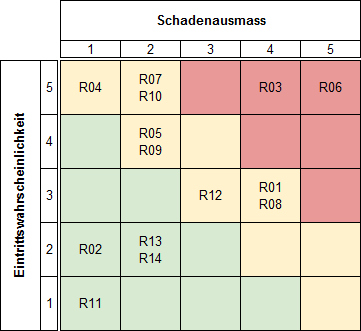
\includegraphics[scale=0.7]{images/risk_result.png}
	\caption{Risiko Matrix}
	\label{Risk result}
\end{figure}

Als Konsequenz kann folgende Aufteilung getroffen werden:
\begin{itemize}
	\item{\textbf{Risiko hoch: } R03, R06}
	\item{\textbf{Risiko mittel:} R01, R04, R05, R07, R08, R09, R10, R12 }
	\item{\textbf{Risiko klein:} R02, R11, R13, R14}
\end{itemize}
\subsection{Massnahmen}
Für die hohen und mittleren Risiken wurden folgende Massnahmen festgelegt:
\begin{itemize}
	\item{\textbf{R03 - Internet auf Mobilgerät:} \\
	\textbf{Massnahmen:} Es muss sichergestellt werden, dass die Drohne nicht auf eine permanente Serververbindung angewiesen ist. Monitor und Datenlogging dürfen kurze Unterbrechungen aufweisen. Die Mission darf aber zu keinem Zeitpunkt gefährdet werden, die Drohne muss selbstständig am Bestimmungsort landen.}
	
	\item{\textbf{R06 - Absturz und Schäden:} \\
	\textbf{Massnahmen:} Bei der Wahl der Drohne wurde auf eine Verfügbarkeit der Ersatzteile geachtet. Ebenfalls wurde darauf geachtet, dass die Bezugsquellen in der Schweiz einen adequaten Lagerbestand aufweisen.}

	\item{\textbf{R01 - JMS auf Mobilgerät:} \\
	\textbf{Massnahmen:} Bei der Evaluierung der Komponenten wird ein JMS Implementierung gewählt, die auf einem Android Betriebssystem lauffähig ist. Dies wird in einem Proof of Concept überprüft.}
	
	\item{\textbf{R04 - Infrastruktur Problme:} \\
	\textbf{Massnahmen:} Auf Grund von Erfahrungen aus früheren Projekten, wird auf die Serverinfrastruktur der HSR verzichtet, dies garantiert eine volle Kontrolle über den Server. Es muss jedoch berücksichtig werden, dass der administrativ Aufwand höher ist und somit mehr Zeit in Anspruch nehmen wird.}
	
	\item{\textbf{R05 - Kapazität der Drohne:} \\
	\textbf{Massnahmen:} Sollte die Drohne nicht ein Gewicht transportieren, dass einer Demonstration würdig ist, wird ein Akkupack mit mehr Spannung angeschaft.}	
	
	\item{\textbf{R07 - Positionsungenauigkeit:} \\
	\textbf{Massnahmen:} Bei Flugkoridoren und Landepunkten genügend Sicherheitsmarge einrechnen, damit die GPS Ungenauigkeit keine unvorhergesehnen Probleme bereiten kann.}
	
	\item{\textbf{R08 - Ardupilot Handhabung:} \\
	\textbf{Massnahmen:} Von Anfang an die gesammte Route an Ardupilot übertragen. Dies muss in einem Proof of Concept genauer eruiert werden.}
	
	\item{\textbf{R09 - Ardupilot API:} \\
	\textbf{Massnahmen:} Früh in einem Proof of Concept die Möglichkeiten und Grenzen des APIs nachvollziehen.}
	
	\item{\textbf{R10 - Entwicklungsprozesse:} \\
	\textbf{Massnahmen:} Bewusster Umgang mit der Resource Zeit. Gegebenenfalls Arbeitsplatz im Freien, um Zeit während des Deployments auf die Drohne zu sparen.}
	
	\item{\textbf{R12 - Ablademanagement:} \\
	\textbf{Massnahmen:} Prüfung einer Abwurfmöglichkeit. Gegebenenfalls Benutzer mit GUI auf Mobile begleiten um einen sicheren und unfallfreien Ablad zu garantieren.}
\end{itemize}

\section{Qualitätsmassnahmen}	
\subsection{Dokumentation}
Die Dokumentation wird vollständig in Latex geschrieben und befindet sich zu jedem Zeitpunkt auf dem Project-Helin github repository: github.com/project-helin.

\subsection{Projektmanagement}
Für das Projektmanagement wird Jira von Atlassian verwendet. \\
Als Projektmanagmenet Methodik wird Scrum verwendet, jedoch werden einige Meilensteine gesetzt um den Fokus nicht aus den Augen zu verlieren und sich über Teilziele bewusst zu sein.

\subsection{Entwicklung}
Die Qualität der Entwicklung wird durch folgende Massnahmen sichergestellt:
\begin{itemize}
	\item{\textbf{Code Review:} Bei kritischen Komponenten werden Code Reviews durchgeführt um sich Designentscheidungen bewusst vor Augen zu führen.}
	
	\item{\textbf{Testing:} Das gesammte Projekt wird in Java entwickelt. Als Unit-Test Framework wird folglich JUnit4 verwendet.}
	
	\item{\textbf{Versionierung:} Der gesammte Quellcode wird mithilfe von github versioniert.}
	
	\item{\textbf{Deployment:} Die Serverkomponenten werden mithilfe eines Build Systems deployt. Die Komponenten auf den Mobiltelefonen werden manuell deployt. Jedoch werden auf dem Build-System ebenfalls Unit-Tests zu Verfügung gestellt.}
	
\end{itemize}


\chapter{Sitzungsprotokolle}
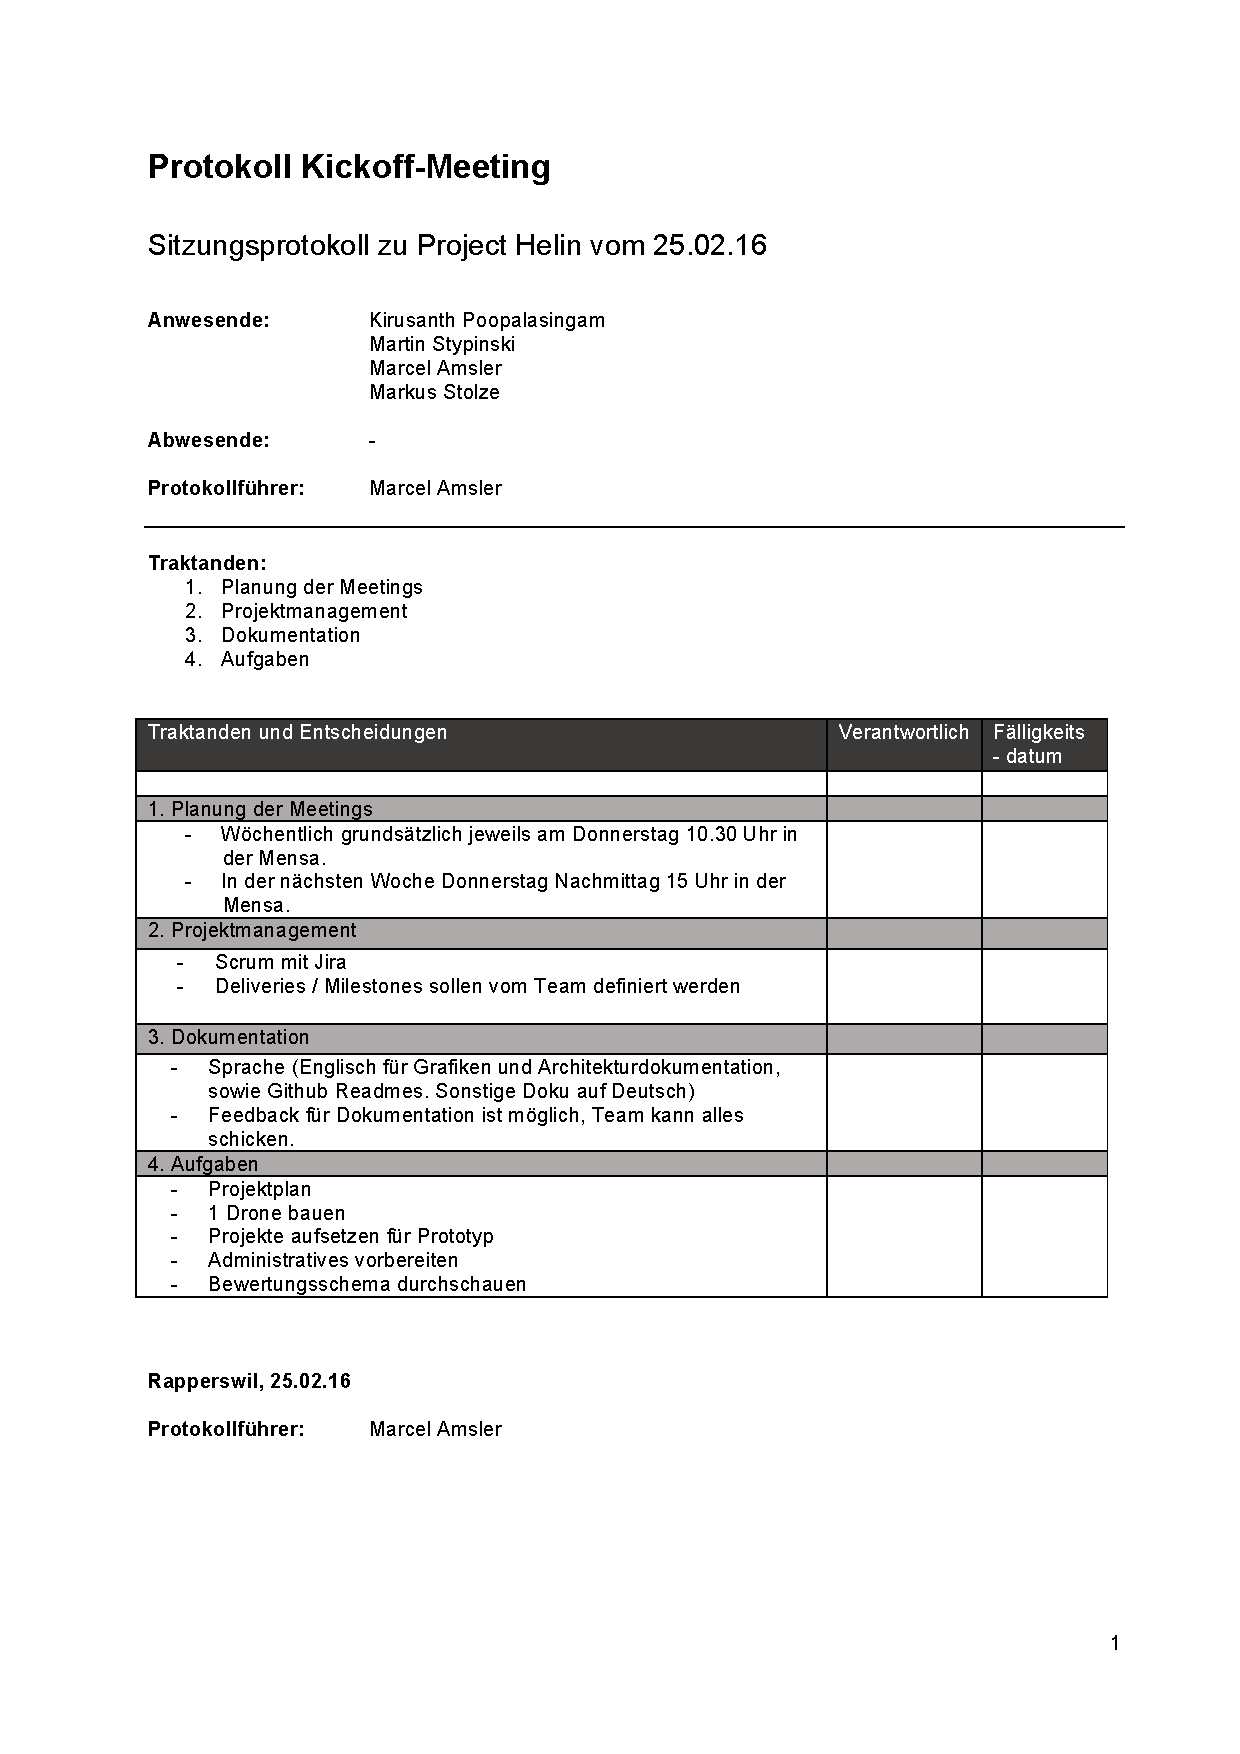
\includepdf[pages=-]{chapter/52protocol/protokoll_w01.pdf} 


% Templates
%%%%%%%%%%%%%%%%%%%%%%%%%%%%
\newpage
\chapter{Demo and Template}
\section{Zitieren}
\begin{itemize}
	\item{So zitiere ich algemein, \cite{lin1973} yo}
	\item{So zitiere ich spezfifisch, \cite[S. 15]{lin1973}}
	\item{So zitiere ich Web... web \cite{learnHaskell}}
	\item{Quelle nachtragen: \textit{index/bibliography.bib}}
\end{itemize}

\section{Glossar}
Ein Eintrag in das Glossar wird wie folgt gemacht:
\begin{itemize}
	\item{\Gls{Clusteranalyse} - wird ins Glassar eingefügt}
	\item{Eintrag in \textit{index/glossar.tex}}
	\item{Es kann sein, dass der Eintrag nicht erscheint. Dann das build script ausführen, damit die Index Dateien neu hinzugefügt werden...}
\end{itemize}

% List of figures & glossary
%%%%%%%%%%%%%%%%%%%%%%%%%%%%

\listoffigures

\clearpage

\printglossary[style=altlist,title=Glossar]

% Bibliography
%%%%%%%%%%%%%%
\bibliographystyle {alpha}
\bibliography{index/bibliography}



\end{document}